In both of our extrapolation frameworks, we deliberately considered every available frequency to predict the ground-state energy, since we wanted to obtain a more general extrapolation. This "black-box" behavior could lead to worse predictions, but does not require a hand-selection of a subset of the sequences for extrapolation. Also, this would require a metric on what sequences to choose. For ground-state energies, the convergence is monotonic and decreasing, such that we \textit{could} choose such a metric, where we choose the three sequences, for which the value at the highest $N_\mathrm{max}$ are the lowest among all sequences available. We want to demonstrate this frequency preselection idea by evaluating the \n{2}{H} nucleus using the same interaction as in the previous chapters with a flow parameter of \srg{0.08}.

In \autoref{fig:eval_freqselection}, the results are shown. If we compare these results to the results of the unmodified training in \autoref{fig:eval_diff} for the \srg{0.08} interaction of \n{2}{H}, we can see that the frequency preselection significantly improves the absolute value, as well as the uncertainty of the prediction for the $N_\mathrm{max}$ values of $8$ and $10$.

Of course, manually selecting the sequences which will be used in evaluation with a predefined metric limits the extrapolation framework to the types of observables for which this metric can apply. For example, after we have decided to only use the sequences with the three lowest values at the highest $N_\mathrm{max}$, the framework gets limited to ground-state energies. The extrapolation of other observables, that do not show the monotone decreasing convergence behavior of the ground-state energy will therefore not be optimized.

In the end, the decision to use a manual preselection of frequency is a tradeoff between a framework with more precise and more accurate predictions and a framework which is more general.

If one decides to manually preselect frequencies for evaluation, it may be of interest to also develop and analyze different metrics for choosing such sequences. In the case of our ground-state energy extrapolation framework, we chose the lowest sequences as the best sequences to choose. Another possibility would be to choose the three sequences which show the most uniform convergence behavior, as we have observed that this significantly lowers the uncertainty in the predictions.

\begin{figure}[H]
  \centering
  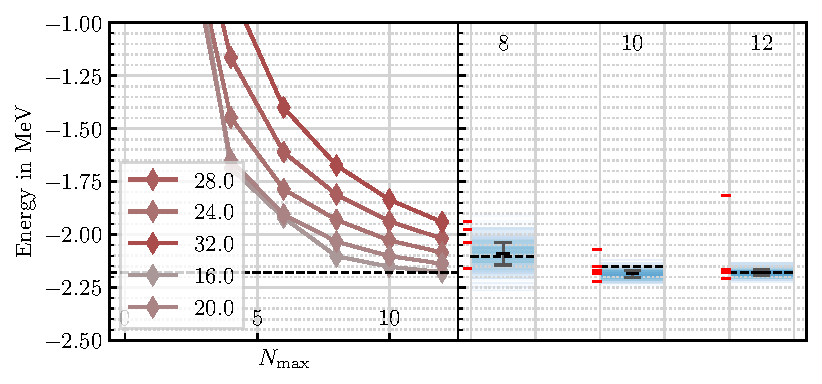
\includegraphics{media/outlook_selection.pdf}
  \caption{Evaluation of the \n{2}{H} nucleus in the difference-based framework using only the three lowest frequencies. In this case, the frequencies are $\hbar\Omega = 16, 20, \SI{24}{\mega\electronvolt}$. The frequencies used in the evaluation are shown with solid lines. To achieve a better comparability to the previous extrapolations, the frequencies not taken into account are shown as dotted lines.}
  \label{fig:eval_freqselection}
\end{figure}
